\chapter{Solving Shortest Path in Traffic Assignment} \label{chap:iterative}
The previous chapter suggests the use of A* search with zero-flow travel times as heuristic estimates and the min-heap priority queue implementation from the C++ standard template library for solving the shortest path problem.

So far we have only been dealing with solving the shortest path problem on static graphs for travel time based on fixed flow.
In this chapter we discuss solving the problem in the path equilibration algorithm where
the graph dynamically changes its arc costs between iterations.
Better performance can be achieved if we are able to use information from previous iterations, for example reusing shortest path from the previous iteration.

\section{Avoiding shortest path calculations} \label{section:avoid}
All of the shortest algorithms mentioned so far need to fully calculate the shortest path between every O-D pair in each iteration.
It turns out for every O-D pair in the path equilibration algorithm,
their shortest path calculation can be avoided to reduce computational time by using solution from the previous iteration in the current iteration.

The basic framework is as follows.
First a complete iteration of the path equilibration algorithm is performed and all of the shortest paths are stored.
Then for every subsequent iterations,
we either perform a shortest path calculation or skip the calculation by some strategy.
If a shortest path is skipped, the stored path from the last iteration is used.

Two situations can occur if we choose to do so.
The first situation is when the shortest path between the previous and current iteration are the same,
then we have successfully avoided the calculation and reduced the computational time.
The second situation is when the paths are different,
then the path equilibration algorithm may not move closer to its equilibrium state after the current iteration,
which causes a possible increase in the total number of iterations and computational time.
Although the total number of iterations may vary,
the path equilibration will still converge.
This is because with a proper defined strategy,
where a new shortest path will be calculated eventually, non-converging iterations will get corrected and converge when new shortest path is calculated.

While traffic flows and arc costs change between iterations,
if we can prove that shortest path do not change often between iterations,
then some strategies can be used to avoid the calculations.
The overall computational time is reduced when most shortest path calculations are avoided on the O-D pairs that are not going to change often.

Figure~\ref{fig:sp_change} shows how often shortest paths change between iterations for the Chicago Sketch and Berlin Center network (details of the networks can be found in Table~\ref{table:problemdata}).
The histogram show the total number of times the shortest path for an O-D pair changed 0,1,2,\ldots, times (in percentage out of all O-D pairs).
The figure shows that on both networks, 60\% and 91\% of all O-D pairs have not changed their shortest path after the initial iteration,
and 16\% and 3\% of all O-D pairs changed their shortest path only once.
This means that after the first iterations,
the algorithm spends most of its time changing only a dozen of O-D pairs' shortest path.
From these observations,
it is assured that run time can be reduced if we avoid shortest path calculations that do not change between iterations.

\begin{figure}[!ht]
    \centering
    \begin{subfigure}{.5\textwidth}
        \centering
        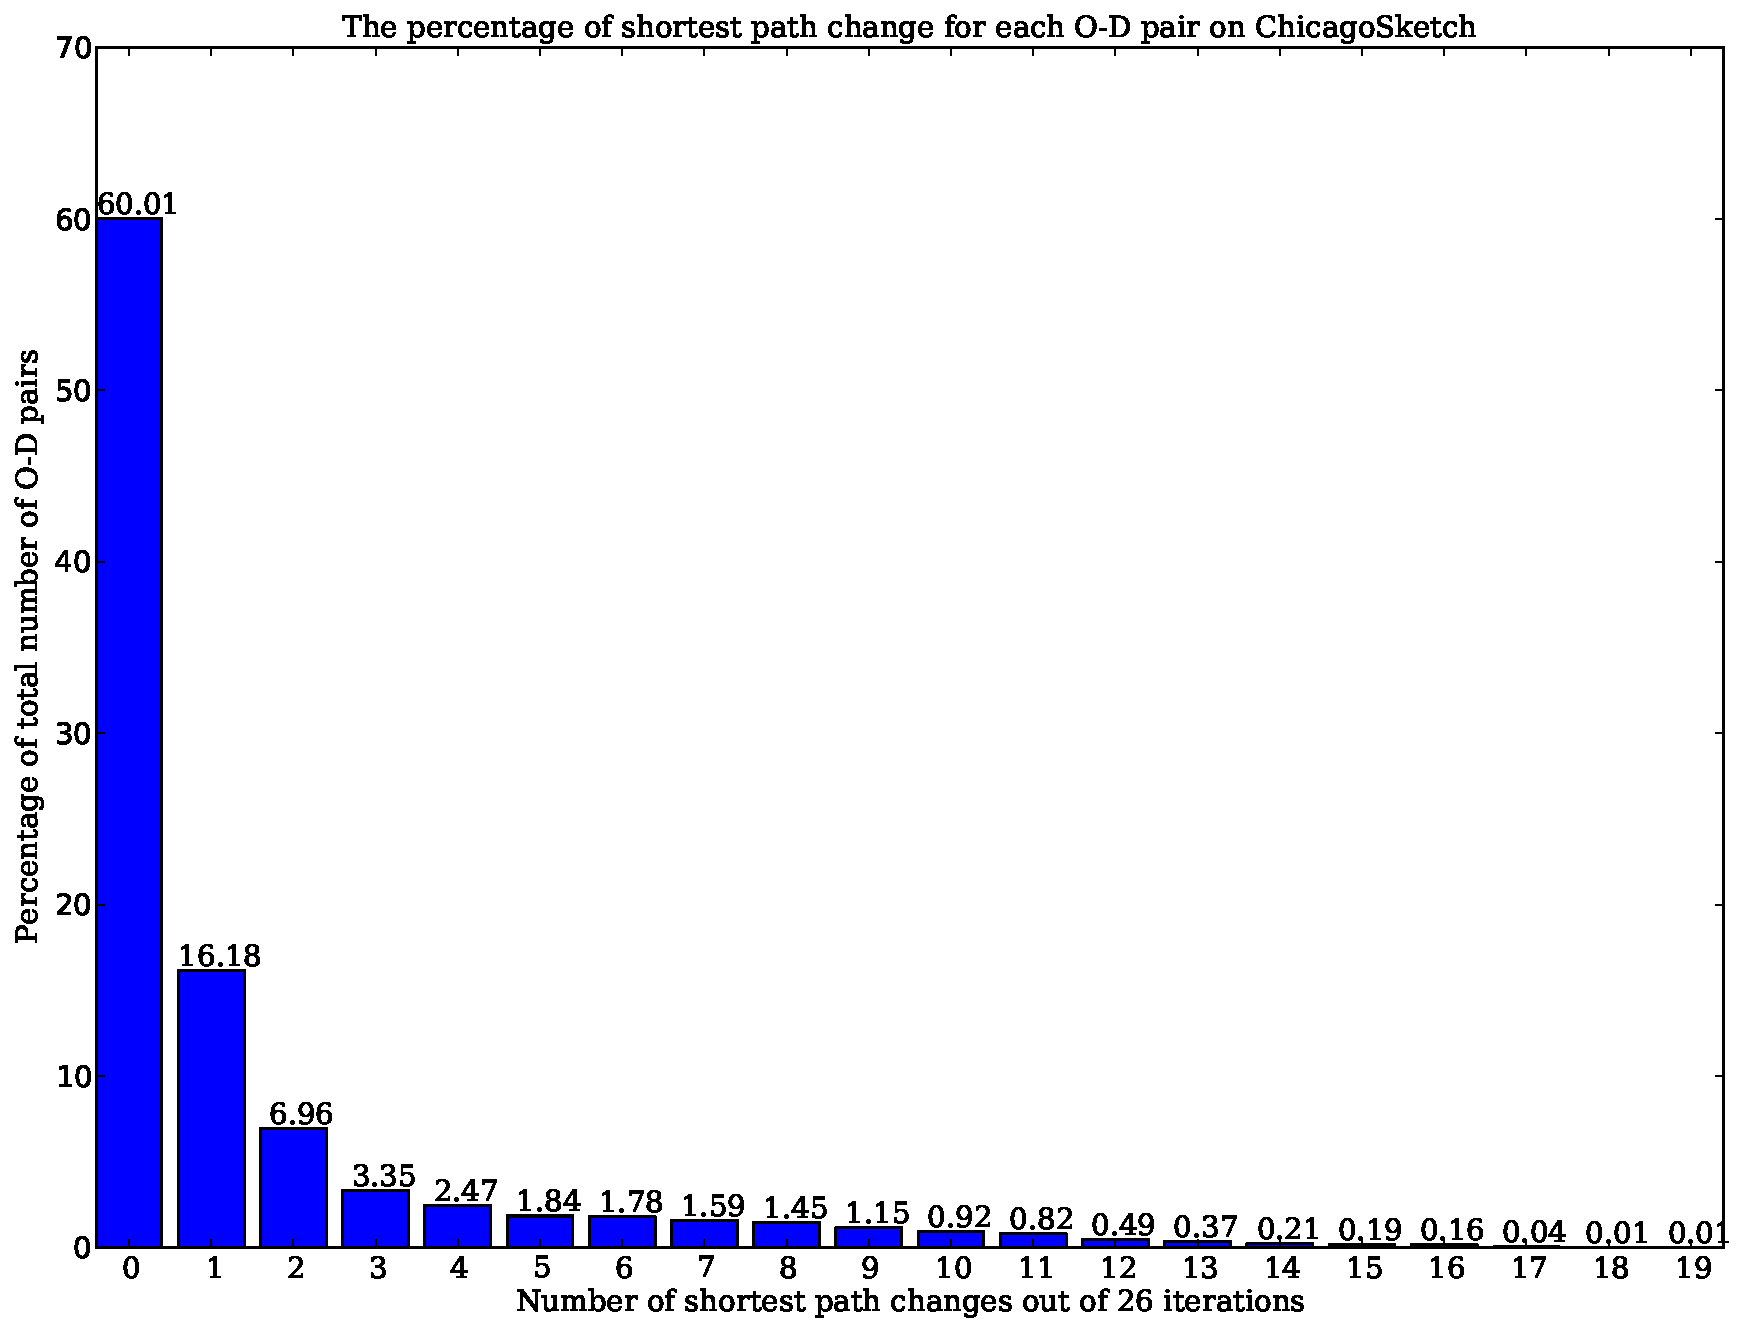
\includegraphics[page=1, width=\textwidth]{img/sp_change}
        \caption{Out of 26 iterations on Chicago Sketch}
        \label{fig:sp_change_chicago}
    \end{subfigure}%
    \begin{subfigure}{.5\textwidth}
        \centering
        \includegraphics[page=2, width=\textwidth]{img/sp_change}
        \caption{Out of 23 iterations on Berlin Center}
        \label{fig:sp_change_berlin}
    \end{subfigure}
        \caption{The percentage of shortest path change for each O-D pair}
        \label{fig:sp_change}
\end{figure}

\subsection{Avoiding a number of iterations}
The first strategy is as follows.
For each O-D pair,
if its shortest path did not change in the last two iterations,
then we can delay the next shortest path calculation by a few iterations.
This strategy requires prior knowledge of how many iterations there is going to be during a standard run.
This is because if we choose to skip more calculations than the total number of iterations,
then there will be excessive iterations resulting in wasted time.
If we skip too few iterations,
then there may not be any impact on the computational time.

This strategy requires to store shortest path between iterations,
memory may become an issue if the number of O-D pairs is large.
This strategy also requires to compare the stored paths when iterations are not skipped and  copy the stored path to the current iteration when iterations are skipped,
this will increase the run time.

\subsection{Avoiding the next shortest path calculation randomly}
The other strategy is to skip shortest path calculations randomly.
That is, when it comes to calculate the shortest path for a given O-D pair,
we generate a random number and decide whether to perform the calculation based on that number.
The advantage of this strategy is that we do not need to know how many iterations the algorithm will take,
and shortest paths do not need to be stored.
The disadvantage is that the computational time can vary between different runs,
resulting in unpredictable run times.

This strategy also requires to store and copy shortest paths between iterations,
but paths do not need to be compared, so this strategy is faster than the first strategy.

\section{Results on avoiding shortest path calculations}
In this section, we consider avoiding shortest path calculations in the iterative path equilibration algorithm using strategies described in the previous sections.
A* search is used to generate results for this section as it is identified to be the most efficient algorithm in Section~\ref{sec:allresults}.

We present the strategy of avoiding a pre-defined number of shortest path calculations for each O-D pair if the previous two iterations result identical shortest path.
The results are shown in Figure~\ref{fig:skip_n},
where the strategy is tested on the Berlin Center and Chicago Sketch network.
On both networks,
we choose to avoid the next 5, 10, 15 and 20 iterations,
these numbers are sensibly chosen because in a normal run of the path equilibration algorithm, it takes 23 and 26 iterations on the Berlin Center and Chicago Sketch network respectively.
The strategy does not work well on the Berlin Center network,
where run time is only decreased slightly when 5 iterations are skipped,
and all other skips increased the run time significantly.
Due to the size of the network,
the run time is heavily affected by the increase in total number of iterations.
The strategy worked well on the Chicago Sketch network.
Skipping 5 iterations resulted the same 26 iterations and the run time is decreased by 4 seconds.
Run times are still reduced in cases where there is an increase in total number of iterations.
Overall the run times become unpredictable when more iterations are skipped.

\begin{figure}[t]
    \centering
    \begin{subfigure}{.5\textwidth}
        \centering
        \includegraphics[page=3,width=\textwidth]{img/random_time}
        \caption{Berlin Center network}
        \label{fig:berlin_skip_n}
    \end{subfigure}%
    \begin{subfigure}{.5\textwidth}
        \centering
        \includegraphics[page=4,width=\textwidth]{img/random_time}
        \caption{Chicago Sketch network}
        \label{fig:chicago_skip_n}
    \end{subfigure}
    \caption{Run time for avoiding shortest path calculations if the previous two iteration did not change}
    \label{fig:skip_n}
\end{figure}


The other strategy is to skip the next shortest path calculation randomly.
%The advantage of this strategy is that it does not need the number of iterations it will compute,
%but the disadvantage is that the run time may vary between different runs.
Figure~\ref{fig:random_n} shows the results on both Berlin Center and Chicago Sketch, where probabilities of 0.3, 0.4, 0.5, 0.6 and 0.7 for skipping the next shortest path calculation are chosen.
All of the probabilities are run 10 times so the average and extremes of the run times can be determined.
On both networks, run times are unpredictable,
there are extremes where run times are increased by 10\% on Berlin Center and 30\% on Chicago Sketch. With 0.7 probability, the run time increased significantly on Berlin Center meanwhile decreased significantly on Chicago Sketch.
Overall, the average run times can be reduced for probabilities 0.3 to 0.6.

\begin{figure}[t]
    \centering
    \begin{subfigure}{.5\textwidth}
        \centering
        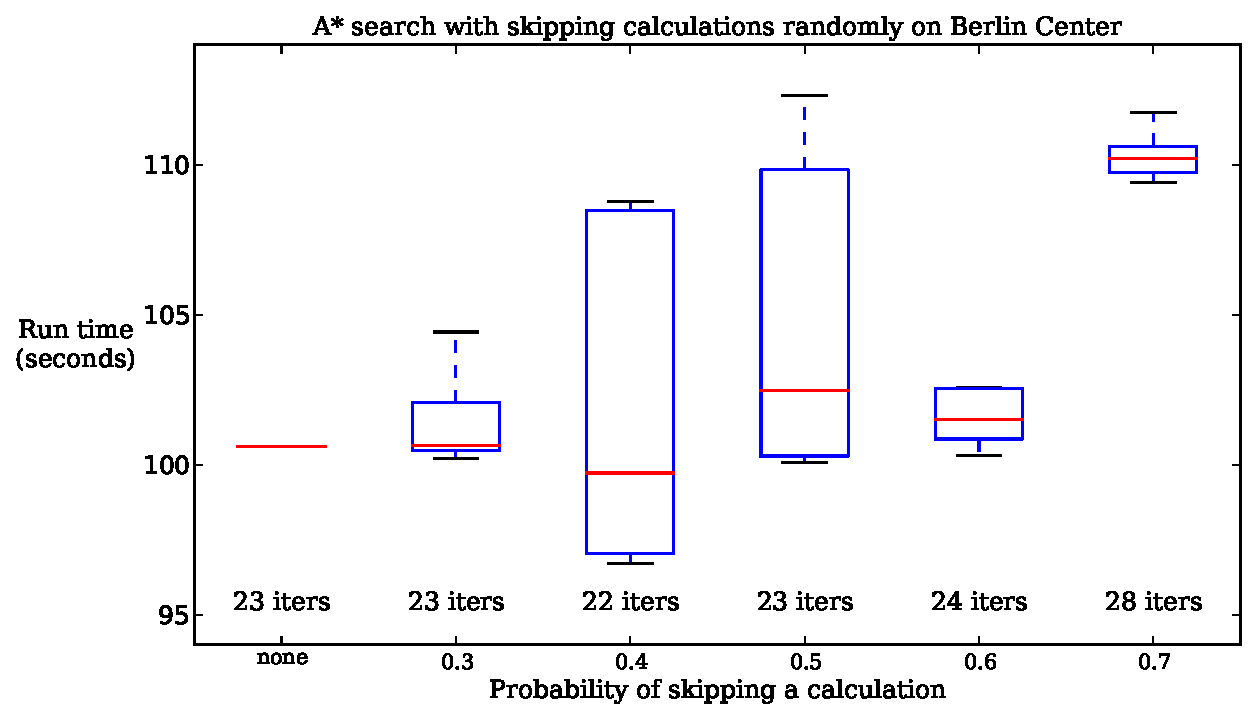
\includegraphics[page=1,width=\textwidth]{img/random_time}
        \caption{Berlin Center network}
        \label{fig:berlin_random_n}
    \end{subfigure}%
    \begin{subfigure}{.5\textwidth}
        \centering
        \includegraphics[page=2,width=\textwidth]{img/random_time}
        \caption{Chicago Sketch network}
        \label{fig:chicago_random_n}
    \end{subfigure}
    \caption{Run time for skipping shortest path calculations randomly}
    \label{fig:random_n}
\end{figure}

%The random strategy can be used before knowing the total number of iterations the path equilibration algorithm going to produce,
The random skipping strategy has a better performance than the other strategy,
and since only small networks have been tested so far,
we now present the random skipping strategy on the Philadelphia and Chicago Regional networks (details in Table~\ref{table:problemdata}) that have over a million O-D pairs.

Due to memory requirement, we switch to a computer with Intel Xeon CPU and 11.7 GiB RAM for the upcoming results.
The run time comparisons are shown in Figure~\ref{fig:large_random_n} (see Table~\ref{table:runtime_large_network} of Appendix~\ref{appendix} for extract results).
The random skipping strategy uses 50\% probability to skip a shortest path calculation.
The strategy has a 25\% and 27\% run time improvement on the Philadelphia and Chicago Regional networks respectively.

\begin{figure}[!hb]
    \centering
    \includegraphics[page=5,width=\textwidth]{img/random_time}
    \caption{Run times of A* search and 50\% random skipping on large networks}
    \label{fig:large_random_n}
\end{figure}

From this chapter, we conclude the following:
\begin{itemize}
    \item the random skipping strategy works well on the tested graphs,
but there are extremes where the algorithm takes significantly longer to run using high probability such as 0.7.
    \item the skipping next few number of iterations strategy works well when just a few iterations are skipped (e.g.\ 5 iterations), the run time becomes unpredictable when more iterations are skipped.
\end{itemize}
